\chapter{Straw Tracking}
\label{chapter:Straw Tracking}
\thispagestyle{myheadings} % should I be including this at the top of every section page??


\graphicspath{ {Body/Figures/TrackingFigures/} {Body/Figures/TrackingFigures/MainPlots/} {Body/Figures/TrackingFigures/MainPlots/PlanePlots/} {Body/Figures/TrackingFigures/MainPlots/PullPlots/} {Body/Figures/TrackingFigures/MainPlots/Residuals/} {Body/Figures/TrackingFigures/eLoss/} {Body/Figures/TrackingFigures/CoordSys/} {Body/Figures/TrackingFigures/TrackerPics/} {Body/Figures/TrackingFigures/Field/} {Body/Figures/TrackingFigures/TrackingFlow/} {Body/Figures/TrackingFigures/LeftRight/} {Body/Figures/TrackingFigures/Misc/}}

\section{Straw Tracking Intro}
\label{sec:StrawTrackingIntro}


  The Muon \gmtwo Experiment at Fermilab uses straw tracking detectors to measure decay positron trajectories for the purpose of determining the muon beam distribution and its characteristics. By fitting these tracks and extrapolating back to the average decay point, the beam can be characterized in a non-destructive fashion. This is important because of the need for matching the average observed magnetic field of the decaying muons and their resulting decay positron directions which result in the \wa frequency, as seen in
        \begin{align} \label{eq:wa}
            \vec{\omega}_{a} = \frac{e}{m} [a_{\mu}\vec{B} - a_{\mu} (\frac{\gamma}{\gamma+1})(\vec{\beta} \cdot \vec{B})\vec{B} - (a_{\mu} - \frac{1}{\gamma^{2}-1})(\vec{\beta} \times \vec{E}) ].
        \end{align}
  The trackers are also useful for determining general beam diagnostics as well as the pitch correction and to a lesser extent the electric field correction, terms 2 and 3 in Equation \ref{eq:wa} respectively. The tracking analysis can be done independently of, or in tandem with, the calorimeters. Cross-checking separately for pileup removal, hit verification, etc. is a powerful tool. Combining them in order to provide the muon distribution that the calorimeters directly see for the \wa calculation is perhaps the most important role of the tracker. (An EDM analysis needs to be done separately.) It is worth noting that there is a large percentage of tracks hitting the calorimeters that hit zero or only a small number of tracking modules, which this Geane fitting code is not capable of handling. With three trackers, approximately 5\% of decaying muons will result in measureable positron tracks assuming no pileup in the tracker, many of which do not hit the nearest calorimeter. Note that the integration of the two detector systems in the code (tracker-calo matching) has just recently been initiated, \href{https://gm2-docdb.fnal.gov/cgi-bin/private/ShowDocument?docid=7514}{DocDB 7514}.

  Each tracker module consists of 4 layers of 32 straws with a stereo angle of 7.5 degrees, the first two ``U'' layers oriented with the tops of the straws at a greater radial position, and the second two ``V'' layers oriented with the bottoms of the straws at a greater radial position. A tracking module is shown in Figure \ref{fig:tracker}. There are 3 tracker stations located at the 0th, 12th, and 18th sections of the ring, counting clockwise from the top most point of the ring where the inflector resides. Figure \ref{fig:WorldCoordSys} shows this. (Station 18 was installed for the commissioning run, with station 0 planned for the fall. Station 12 might or might not be installed sometime in the future.) Each station consists of 8 tracking modules arranged in a staircase pattern that follows the curvature of the ring as seen in Figure \ref{fig:staircase}. Further hardware and electronics information regarding the trackers will be omitted in this document.

\begin{figure}[]
\caption{Shown is a picture of one of the many tracking modules used in the Muon \gmtwo experiment. The first layer of straws with a stereo angle of 7.5 degrees can be seen, with the other 3 straw layers hiding behind it. The beam direction is roughly into the page in this picture, to the left of the end of the module, and this view is what the decay positrons will see. Picture provided by James Mott.}
\centering
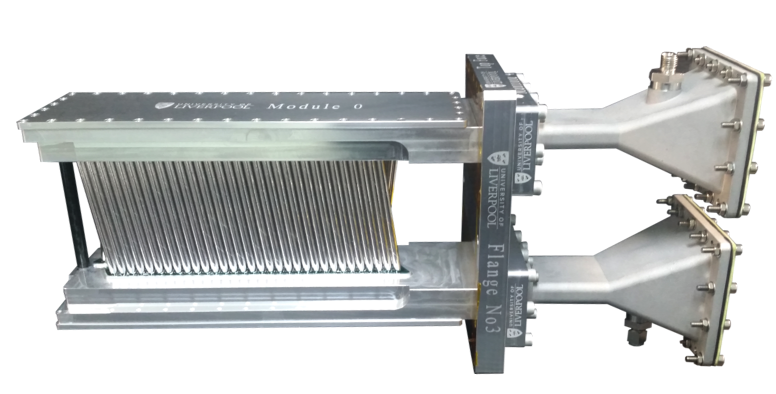
\includegraphics[width=0.9\textwidth]{Tracker}
\label{fig:tracker}
\end{figure}

\begin{figure}[]
\caption{Tracker modules are arranged in the shown staircase pattern. In green and dark blue is the edge of the vacuum chamber (where the dark blue identifies the modification that was made to the old vacuum chambers), and it can be seen that vacuum chamber walls lie at the ends of the outside tracking modules. The position of a calorimeter can be seen in cyan at the right. The dark red spots are the locations of the outside magnet pole tips. From the shown geometry one can see that many positrons will hit either the tracker or the calorimeter but not both due to the acceptance differences.}
\centering
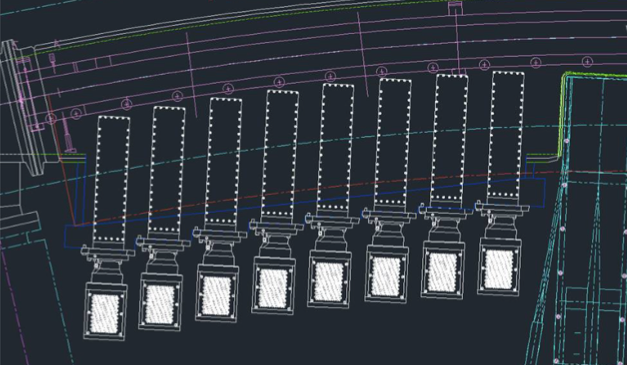
\includegraphics[width=0.9\textwidth]{trackerStation}
\label{fig:staircase}
\end{figure}


  Because of the proximity of the trackers to the muon beam, they will lie within a region of varying magnetic field. The radial field of the trackers rises from 0 Tesla at the outer ends to roughly .3 Tesla at the inner top and bottom ends, and the vertical field drops approximately 50\% from the storage dipole field of 1.451 Tesla. Shown in Figures \ref{fig:operaBy} and \ref{fig:operaBx} is the location of the tracker with respect to the horizontal and vertical fields respectively. These large field gradients over the tracking detector region and the long extrapolation distance back to the muon decay point are special to Muon \gmtwo. This is one of the main motivations for using the Geane (Geometry and Error Propagation) fitting algorithm and routines, which has direct access to the field. 


\begin{figure}[]
\caption{Shown is the vertical field of the \gmtwo magnet in and around the storage region as calculated in Opera 2D. The center of the storage region lies at 7.112 m along the x axis. The black box shows the rough location of the tracker with respect to the field (size exaggerated slightly). It can be seen that there is a large inhomogeneity within the tracker space, goring from left to right.}
\centering
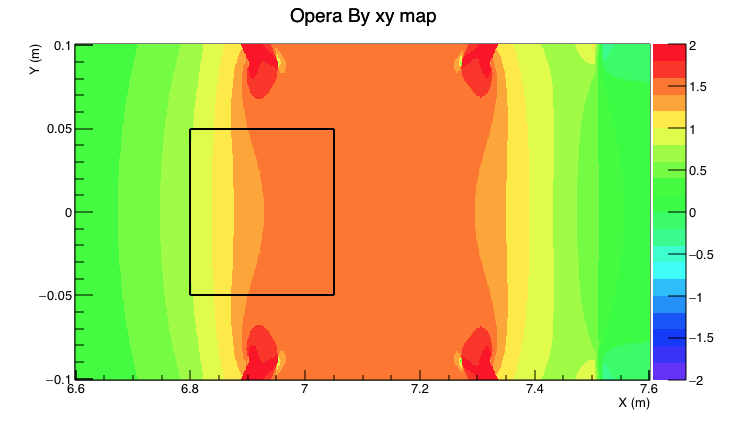
\includegraphics[width=0.9\textwidth]{operaBy}
\label{fig:operaBy}
\end{figure}

\begin{figure}[]
\caption{Shown is the radial field of the \gmtwo magnet in and around the storage region as calculated in Opera 2D. The center of the storage region lies at 7.112 m along the x axis. The black box shows the rough location of the tracker with respect to the field (size exaggerated slightly). It can be seen that there is a large homogeneity at the inner upper and lower ends compared to the right center. The shape of the pole pieces and tips can readily be seen.}
\centering
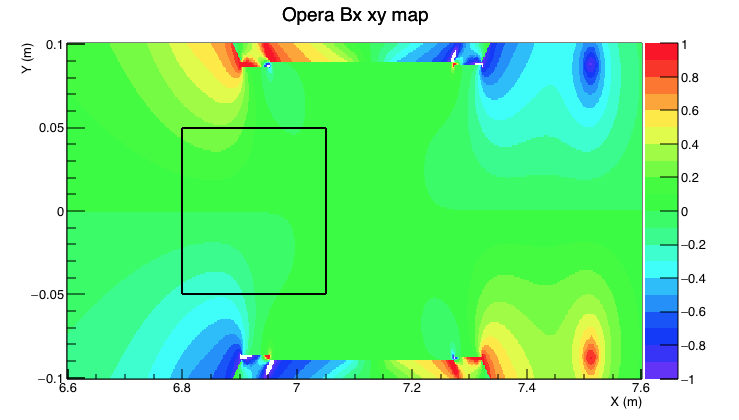
\includegraphics[width=0.9\textwidth]{operaBx}
\label{fig:operaBx}
\end{figure}

  The Geane fitting routines originated in Fortran with the EMC collaboration, and was used in the precursor E821 experiment as well as the PANDA experiment with some success \cite{geanemanual}, \cite{Lavezzi}. (I'm not actually aware of a useful reference for it's use in E821, and there are some other instances of its use as well in other experiments. In E821 there was a single tracking chamber which was never put to full use.) The core error propagation routines were at some point added to Geant4 under the error\_propagation directory which is included in all default installs. The tracking code strengths lie with its direct implementation and access to the Geant4 geometry and field, and its ability to handle the field inhomogeneties. The Geane fitting algorithm code which makes use of the Geant4 error propagation routines follows the structure of \cite{geanemanual} and is detailed in the \hyperref[sec:Formalism]{Formalism} section in this paper. It is a relatively straight forward least squares global \chisq minimization algorithm. 








\section{Track Finding}
\label{sec:Track Finding}

\section{Track Fitting}
\label{sec:Track Fitting}

\section{Track Extrapolation}
\label{sec:Track Extrapolation}
